

\vspace*{\fill}
\textbf{Proyecto Web en Ruby on Rails}
\vspace{5em}
\begin{center}
	
\includegraphics[scale=0.5]{imagenes/ruby.jpg} 
\end{center}
	
\vspace*{\fill}


\newpage 
	
\vspace*{\fill}
\begin{center}
		
                        
\includegraphics[scale=1.5]{imagenes/ruby.jpg} 
	\end{center}
	
			\begin{center}
				Manual de Usuario \\
				\vspace{5em}
				\Huge{\textbf{``Ruby on Rails''	\vspace{3em}}}
			\end{center}	
			
			


				\hspace*{5cm}Desarrollador:
				\\\hspace*{8cm}Dennise Pintado


\vspace*{\fill}
\newpage 


\section{Introducción}
En este proyecto se trabajó con Ruby on Rails un framework de aplicaciones web de código abierto escrito en el lenguaje Ruby.El mismo es un entorno de desarrollo web que esta optimizado para la satisfacción de el mundo de programadores y tiene una alta eficiencia y rapidez, dejándonos ver con poco el modelo vista controlador.Está optimizado por lo cual evita que utilices código repetitivo en tu proyecto y sigue las reglas básicas de estilo y páginas web como son html y css.
Con ayuda de un conjunto de librerías, automatismo y convenciones que resuelven problemas comunes a la hora de desarrollar. se nos ha pedido crear una página web haciendo uso de CRUD y de MVC,con el afán de poder conocer un poco de este lenguaje.

\section{Alcance}
El proyecto realizado es una página web que muestra el listado de los estudiantes de Ingenieria en Computacion y sus materias respectivas. Consta de tres páginas principales una en la que se muestra en Home o la pantalla de inicio , en la otra se muestra la lista de los estudiantes en una tabla con opcion de eliminar, editar o ver el estudiante que se seleccione y también con una opción extra de crear estudiantes. También consta en la opción de ver o editar, una subsección en donde podemos ver que materia corresponde al código mostrado en la tabla, para saber que materia se encuentra viendo el estudiante.En la tercera pantalla principal se muestra la misión y la visión de la Carrera de Ingenieria en Computacion.

En la primera pantalla se tiene un header que se hizo utilizando sass el css que contiene ruby y las imagenes proyectadas se encuentran en la carpeta de imagenes en assets. Se creo un menu horizontal para las tres páginas principales y se hizo uso de efectos con el mouse y layouts propios de sass y css.Las imagenes tomadas corresponden a la pagina ilustracion online de donde se selecciono de acuerdo a lo que se necesitaba proyectar,y se fuciono haciendolo una portada. La segunda pantalla tiene como objetivo enlistar a los estudiantes , en esta tenemos tres columnas donde llevan los nombres, los apellidos y las materias que toman los alumnos y en tres columnas extras las opciones editar, eliminar y ver.La tercera pantalla principal se trata de la carrera como mencionamos su vision y mision y se hace uso de la imagen proyectada en la pagina web de la FIEC.

\section{Experiencias y Conclusiones}
Para la creacion del proyecto se utlizo la guia de instalacion oficial l, para lo cual a medida que se avanzaba en el proyecto se requirio instalar nuevas gemas una para el sqlite otra para el sass, en micaso me toco hacer eso(incluso instale la gema susy que me servia para acomodar mis layouts). Despues de tener instalado el ruby on rails(y haber leído un n número de tutoriales porque los pasos no salieron tal como esperaba), por fin se pudo ver la página de inicio “Welcome aboard”, una gran satisfacción con el comando rails s.

\begin{figure}
\centering
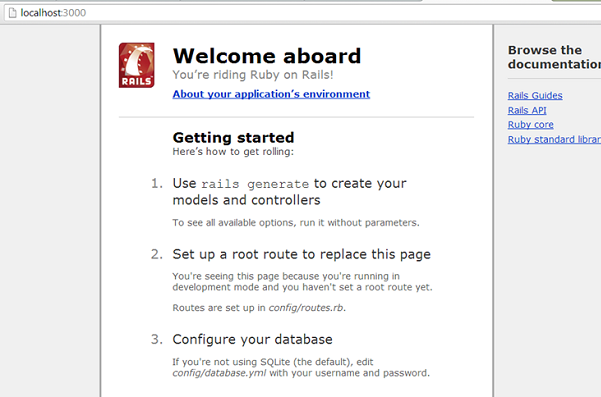
\includegraphics[scale=0.8]{imagenes/rails0.png}
\caption{Welcome aboard Ruby on Rails}
\label{fig: threadsVsSync}
\end{figure}

 Una vez dentro se fue conociendo la estructura , algo muy organizado por lo que ruby sabe donde tiene que acceder para tomar algo en especifico como un  view o un layout o una imagen. Una vez conocida la ruta de la pagina que me mostraba ruby por default, comencé a hacer las pruebas, editando el welcome/index y asu vez conocí el router donde se guardan los accesos de la páginas del proyecto. Avanzando poco a poco, comenzamos con la base por default viene la sqlite, por línea de comando se generó la primera tabla de mi aplicacion web y se introdujo los parámetros de la misma, creada la tabla se generó el helper con los CRUD de cada dato que le generara. También se creó una consulta estática, que tiene datos almacenados en el formulario por get donde se tienen los códigos de la materia de Ingeniería en computación.
Los estilos se los hizo por medio de Sass que es parecido al css, se pueden crear clases y id en el html de la carpeta view, y se edita los valores que se desea que muestre.

\begin{figure}
\centering
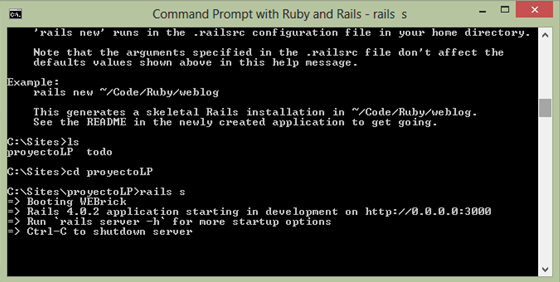
\includegraphics[scale=0.8]{imagenes/rails1.png}
\caption{Conectando con el Server}
\label{fig: threadsVsSync}
\end{figure}

\begin{figure}
\centering
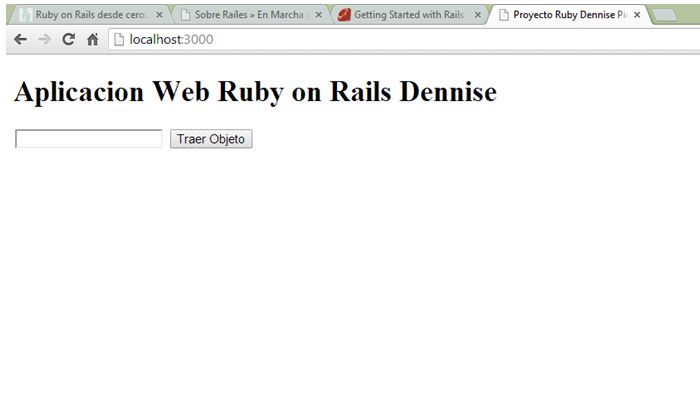
\includegraphics[scale=0.8]{imagenes/rails2.png}
\caption{Primera pagina index}
\label{fig: threadsVsSync}
\end{figure}


\begin{figure}
\centering
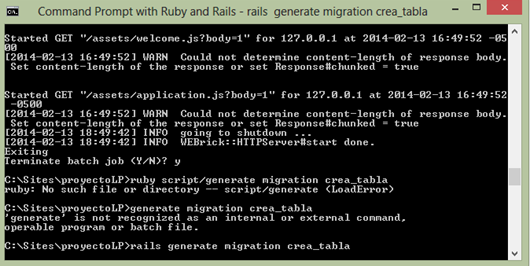
\includegraphics[scale=0.8]{imagenes/rails4.png}
\caption{Creacion de la Base}
\label{fig: threadsVsSync}
\end{figure}

\begin{figure}
\centering
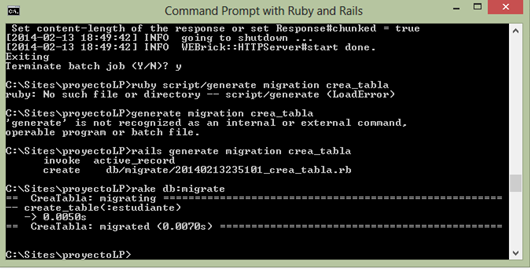
\includegraphics[scale=0.8]{imagenes/rails5.png}
\caption{Migracion de la Base}
\label{fig: threadsVsSync}
\end{figure}

\begin{figure}
\centering
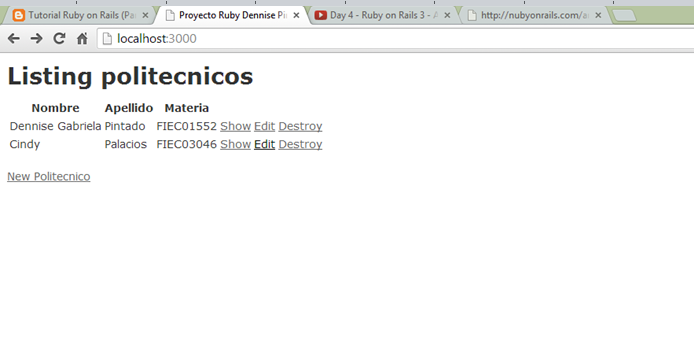
\includegraphics[scale=0.8]{imagenes/rails8.png}
\caption{CRUD de la Base}
\label{fig: threadsVsSync}
\end{figure}
\newpage

En conclusión la herramienta da muchas facilidades, al momento de crear el MVC este ya esta configurado para hacerlo. Personalmente lo más difícil fue el proceso de instalarlo correctamente, puede que esto sea muy trivial pero por algún motivo no lograba llegar a mostrar la página de inicio , tuve que instalar Node.js no se si sea lo común hacerlo peor solo un manual me dijo que debía. Una vez instalado por dentro Ruby esta muy bien sectorizado es decir supe donde encontrar mis vistas y no debía ser explícita con el lenguaje ya que lo hace todo muy automático. Al principio trabajar con las líneas de código puede resultar engorroso , pero a la final uno se  da cuenta que con una línea está creando el mismo código que tomaría semanas en un IDE. La experiencia fue muy interesante el mundo web cambia continuamente y esta herramienta esta sonando mucho a nivel de aplicaciones, me gusto aprender de este framework con esta aplicacion web que tomó menos de lo que podía pronosticar.

\begin{figure}
\centering
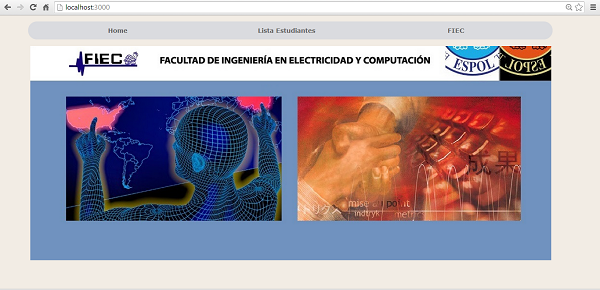
\includegraphics{imagenes/pantallahome.png}
\caption{Pantalla Principal}
\label{fig: threadsVsSync}
\end{figure}

\begin{figure}
\centering
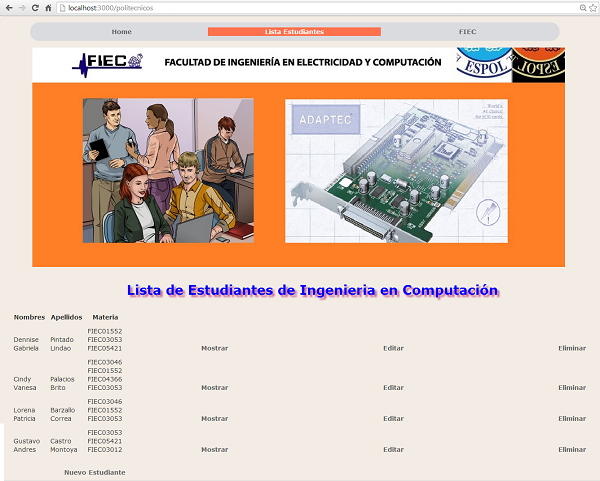
\includegraphics[scale=0.8]{imagenes/pantallalista.png}
\caption{Pantalla Lista de Estudiantes}
\label{fig: threadsVsSync}
\end{figure}


\begin{figure}
\centering
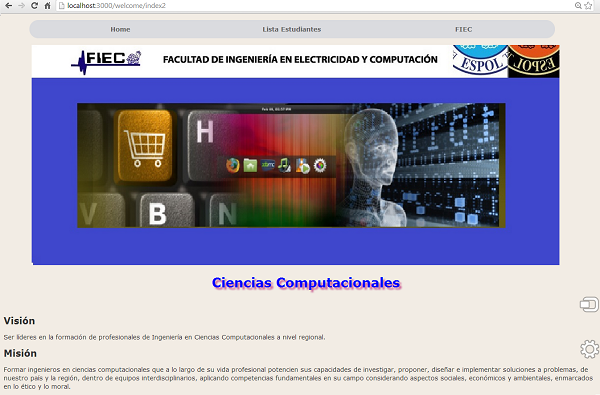
\includegraphics[scale=0.8]{imagenes/pantallafiec.png}
\caption{Pantalla FIEC}
\label{fig: threadsVsSync}
\end{figure}


\begin{figure}
\centering
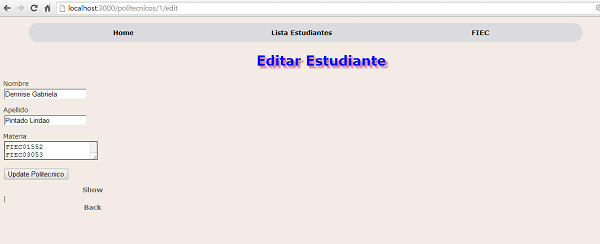
\includegraphics[scale=0.8]{imagenes/editar.png}
\caption{Editar Estudiante}
\label{fig: threadsVsSync}
\end{figure}

\begin{figure}
\centering
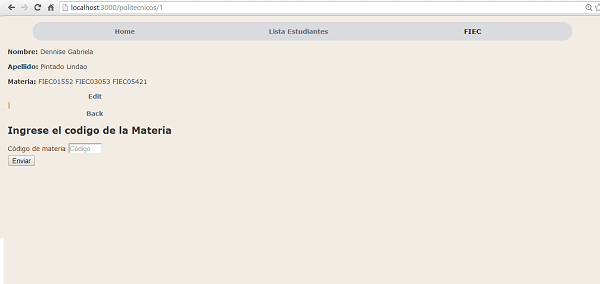
\includegraphics[scale=0.8]{imagenes/mostrar.png}
\caption{Mostrar Estudiante}
\label{fig: threadsVsSync}
\end{figure}

\begin{figure}
\centering
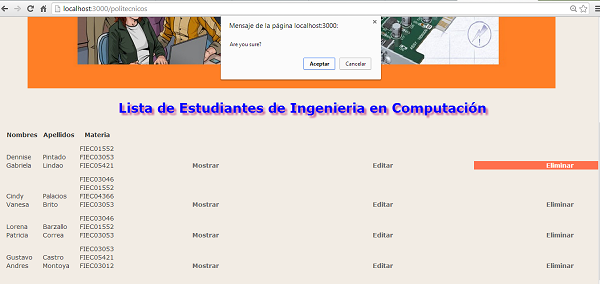
\includegraphics[scale=0.8]{imagenes/eliminar.png}
\caption{Editar Estudiante}
\label{fig: threadsVsSync}
\end{figure}

\begin{figure}
\centering
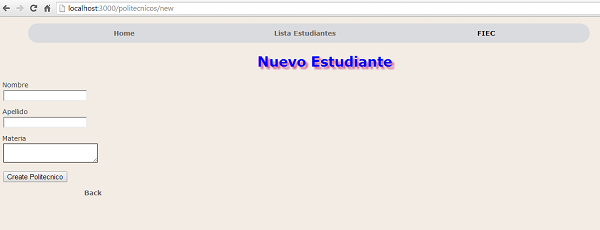
\includegraphics[scale=0.8]{imagenes/nuevo.png}
\caption{Editar Estudiante}
\label{fig: threadsVsSync}
\end{figure}


\newpage
\section{Bibliografía}

\begin{thebibliography}{99}
\bibitem{GuiaRuby}http://guides.rubyonrails.org
\bibitem{ImagenesPortada}http://www.illustrationonline.com/
\bibitem{tutorialRuby}http://www.rubyyyo.com/
\bibitem{tutorialRubyonRails}http://html5facil.com/tutoriales/ruby-on-rails-desde-cero-primeros-pasos
\end{thebibliography}
